\section {Важные с точки зрения влияния на ОС функции}
В различных версиях Windows существует множество динамических библиотек. К базовым обычно относят:
\begin {itemize}
	\item ntdll.dll --- экспортирует так называемые ''родные`` (англ. Native API) функции ядра (набор функций, реализуемых ядром операционной системы - обычно ntoskrnl.exe);
	\item kernel32.dll --- экспортирует функции, отвечающие за управление памятью, вводом-выводом, управление процессами/потоками, однако является в основном лишь ''обёрткой`` над родными API функциями из ntdll.dll;
	\item user32.dll --- высокоуровневую библиотеку для управления графическим интерфейсом;
	\item gdi32.dll --- низкоуровневую библиотеку рисования.
\end {itemize}
Также в контексте работы вредоносного ПО важное значение имеют такие библиотеки, как sfc_os.dll - отвечает за Windows File Protection (функцию защиты от перезаписи важных системных файлов), pstorec.dll - реализует доступ к управляемому Windows защищённому хранилищу паролей.

Большая часть интересующих нас функций, которые будут использовать исследуемые образцы, находится в обычно в kernel32, однако возможно и прямое импортирование  из ntdll, однако ситуации, когда такое может происходить, довольно специфичны --- например, легальное применение Native API обычно присутствует только в антивирусных продуктах.
В процессе запуска исполняемых файлов одним из значимых событий является создание новых процессов, особенно в случае слежения за образцов с помощью отладчика, т.к. все действия, происходящие в новом процессе, не будут отслежены без специальных действий. Также большое значение в действиях вредоносного ПО имеет манипуляция файлами на инфицированном ПК, например, удаление. Далее будут описаны в качестве примера механизмы удаления файла и создания процесса в Windows.

\subparagraph {Удаление файлов}
Как мы можем видеть на рис.\ref{fig:filedelete}, у пользовательских программ есть 2 основных пути
для удаления файлов:
\begin {figure}[h]
	\centering
	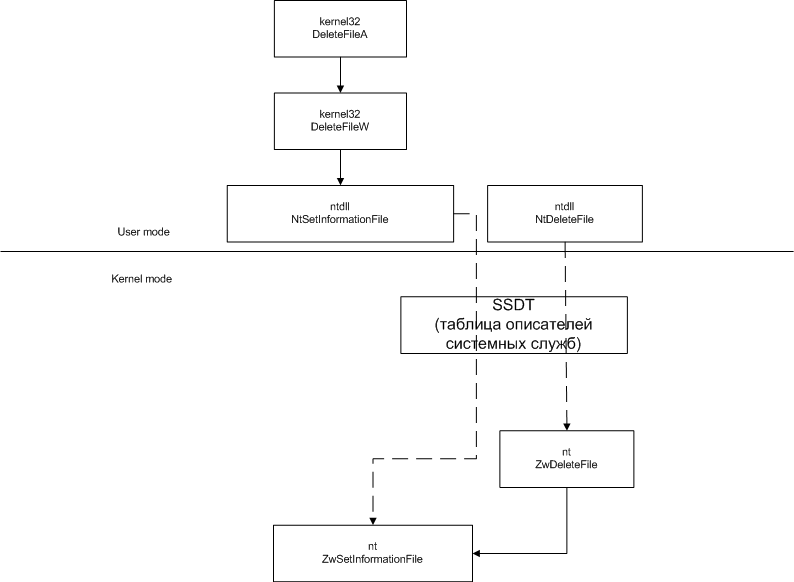
\includegraphics[width=\linewidth]{img/DeleteFileAPIs.png}
	\caption{Функции, отвечающие за удаление файлов}
	\label{fig:filedelete}
\end {figure}
Из схемы следует, что в результате запроса об удалении файла ОС всего лишь помечает атрибуты объекта файла на удаление, а само удаление выполняется другим механизмом. Однако, существуют и другие способы удаления файлов. Например, если файл был создан функцией CreateFile с флагом FILE_FLAG_DELETE_ON_CLOSE, он будет удалён после закрытия все хэндлов и удаления всех ссылок на него без дополнительных обращений из режима пользователя (это пример техники, используемой вирусами для уничтожения следов после осуществеления вредоносной деятельности в системе).
\subparagraph {Создание процессов}
Для создания процессов есть множество различных путей, в том числе, и за рамками приводимых API функций, и нельзя полагаться, что любой создаваемый процесс будет обнаружен, если следить только за ними
\begin {figure}[h]
	\centering
	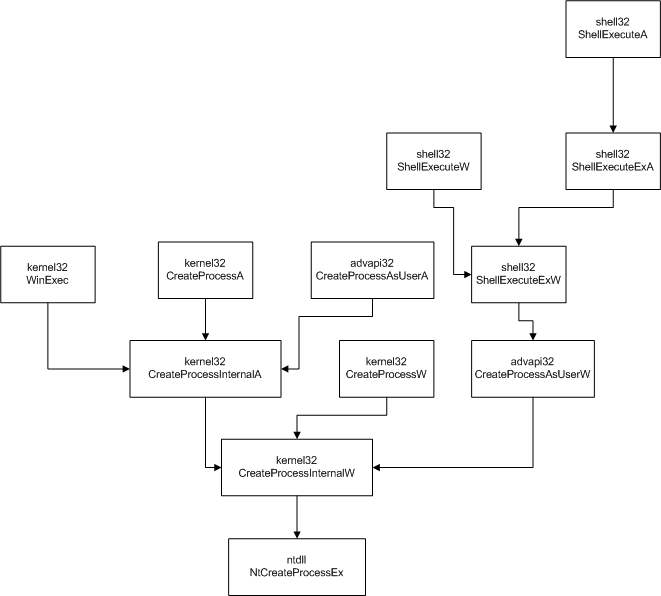
\includegraphics[width=\linewidth]{img/ExampleProcessCreateAPIs.png}
	\caption{Функции, отвечающие за создание процесса}
	\label{fig:createprocess}
\end {figure}